\documentclass[runningheads]{llncs}

\usepackage[T1]{fontenc}
\usepackage[utf8]{inputenc}
\usepackage[english]{babel}
\usepackage{amsmath,amssymb}
\usepackage{graphicx}
\usepackage{booktabs}
\usepackage{hyperref}
\usepackage{makecell}
\usepackage{float}
\graphicspath{{figures/}}

\hypersetup{hidelinks}

\begin{document}

\title{Deep Fuzzy Feature Learning Based on ANFIS for Interpretable Intelligent Systems\thanks{The research was carried out within the state assignment of Ministry of Science and Higher Education of the Russian Federation (theme No. 124112200072-2).}}
\titlerunning{Deep Fuzzy Feature Learning Based on ANFIS}

\author{
    A. N. Averkin\inst{1}\orcidID{0000-0003-1571-3583} \and
    Yu. V. Trofimov\inst{2,3}\orcidID{0009-0005-6943-7432} \and
    A. D. Lebedev\inst{2}\orcidID{0009-0001-1046-5982} \and
    M. D. Lebedev\inst{4}\orcidID{0009-0005-1459-9119} \and
    A. S. Ilin\inst{5}\orcidID{0009-0007-9599-4958} \and
    A. V. Nechaevskiy\inst{2,3}\orcidID{0000-0001-6751-8195}
}

\authorrunning{A. N. Averkin et al.}

\institute{
    Federal Research Center ``Computer Science and Control'' of the Russian Academy of Sciences, Moscow, Russia
    \and Dubna State University, Dubna, Moscow Region, Russia
    \and Joint Institute for Nuclear Research, Dubna, Moscow Region, Russia\\
    \email{ura\_trofim@bk.ru, nechav@uni-dubna.ru}
    \and National University of Science and Technology MISIS, Moscow, Russian Federation
    \and Innopolis University, Innopolis, Russian Federation
}

\maketitle

\begin{abstract}
This paper studies how to increase complexity in neuro-fuzzy models while preserving structural interpretability of internal inference. We design, mathematically formalize, and implement four ANFIS-based architectures in a unified framework: shallow, stacked, hierarchical, and Deep Fuzzy Feature Learning (DFFL). Evaluation is performed across three criteria: predictive quality, rule-base complexity, and reproducibility of internal rule activation across independent runs. In the main comparison block, stacked shows the strongest average-rank profile. DFFL is competitive on selected tasks and exposes a distinct quality--complexity--stability operating point. On full \textit{covtype\_binary}, a large-scale capacity check shows that increasing stacked capacity, adding a gated raw-feature skip, and applying error-focused fine-tuning raises F1 to $0.9466\pm0.0015$, while still remaining below tree ensembles. On the same task, a three-seed DFFL run reaches F1 $=0.8478\pm0.0037$ and remains below stacked and tree ensembles. The results establish an explicit architectural trade-off between predictive quality, structural cost, and reproducibility of internal rule structure.
\keywords{deep fuzzy feature learning \and neuro-fuzzy systems \and interpretable machine learning \and fuzzy inference \and deep learning}
\end{abstract}

\section{Introduction}

Deep models show strong predictive performance on tasks with complex nonlinear structure, yet their internal logic often remains difficult to interpret~\cite{lecun2015deep}. In many applied scenarios this becomes a direct practical constraint. When a model is used for engineering analysis, monitoring, or decision support, experts need to see the reasoning path that leads to the final prediction and the prediction itself~\cite{rudin2019stop}. For this reason, interpretability is treated here as a structural property of the model.

Neuro-fuzzy methods keep their relevance because they combine data-driven learning with explicit rules and membership functions~\cite{jang1993anfis,mitra2000neurofuzzy}. Within this line, ANFIS remains a key reference model due to its combination of adaptive training and readable inference structure~\cite{jang1993anfis}. At the same time, classical ANFIS is shallow by design. As input dimensionality and interaction complexity increase, the rule base grows quickly and becomes harder to preserve in a coherent form~\cite{mitra2000neurofuzzy,magdalena2019semantic}.

This leads to the core question of the study. We need to increase architectural complexity while preserving semantic transparency of internal representations. A simple stacked composition of fuzzy blocks can improve predictive quality, but hidden states in such systems may turn into technical latent transformations instead of interpretable concepts. Hierarchical constructions constrain rule growth more effectively, yet they do not automatically produce semantically transparent intermediate states. As a result, deeper neuro-fuzzy models should be assessed through the way they reorganize internal inference structure, not through expressive capacity alone.

Under these conditions, RMSE or F1 by themselves are not sufficient. It is necessary to evaluate whether internal representations remain interpretable, how stable these representations are across independent runs, and what structural cost is required to maintain them~\cite{rudin2019stop,zeng2019deep,feng2020highly,alvarez2018self,koh2020concept,chen2019looks,chen2020concept}. This viewpoint is especially important for repeated expert review, rule auditing, and decision-support workflows. If predictive quality remains similar but the internal rule structure changes strongly from run to run, then analytical reliability of the model decreases.

The study contribution is concrete and technically explicit. First, we design, mathematically formalize, and implement four ANFIS-based architectures in one unified framework: shallow, stacked, hierarchical, and DFFL. The first three are controlled architectural variants built on established organization principles, while DFFL is introduced as the main concept-oriented architecture with explicit staged concept flow and re-estimation. Second, we evaluate all four architectures under matched preprocessing and optimization settings, which enables a controlled architecture-level comparison rather than fragmented model-by-model tuning. Third, we report a multi-criteria protocol that jointly covers predictive quality, rule-base complexity, and reproducibility of internal rule activation, and we complement it with a case-level internal trace.
The central result is a rigorous architectural comparison that quantifies the quality--complexity--stability trade-off and identifies distinct operating regimes for shallow, stacked, hierarchical, and DFFL designs.

\section{Related Work}

Work in this area starts from classical neuro-fuzzy systems, above all ANFIS, where adaptive learning is coupled with explicit fuzzy inference and preserves a direct relation between model parameters and interpretable rules~\cite{jang1993anfis}. Early surveys described this explicit rule-based structure as the main strength of the approach, while also showing that transparency degrades as task complexity grows~\cite{mitra2000neurofuzzy}.

Hierarchical fuzzy systems were developed as a response to this limitation. Their main goal is to reduce combinatorial rule growth through decomposition of the input space into local subsystems~\cite{magdalena2019semantic,razak2022hierarchical}. This step is important because it shifts the interpretability discussion from separate rules to architectural organization. Yet compact structure alone does not guarantee semantically clear intermediate states.

The next step was the design of deeper rule-based classifiers that keep interpretability constraints. In these models, multilayer processing is combined with low-order rules to retain readability while increasing expressive capacity~\cite{zeng2019deep,feng2020highly}. The reported results confirm that depth and rule-based inference can be combined, but they also show that hidden layers do not become interpretable automatically even when the model remains rule-based~\cite{feng2020highly}.

In parallel, a broader stream of architecturally interpretable deep learning developed outside the neuro-fuzzy line. Self-explaining neural networks treat interpretability as an intrinsic model property~\cite{alvarez2018self}. Concept bottleneck models force prediction to pass through explicit human-readable concepts~\cite{koh2020concept}. Related ideas appear in prototype-based networks and concept-oriented representation learning, where hidden spaces are aligned with representative examples or predefined semantic directions~\cite{chen2019looks,chen2020concept}.

Together, these directions indicate a wider shift from post hoc interpretation toward models with built-in interpretability mechanisms. This distinction is critical because post hoc tools such as LIME and SHAP can explain a trained predictor locally, but they do not guarantee stable and semantically structured internal representations~\cite{ribeiro2016lime,lundberg2017shap,rudin2019stop}.

At the intersection of these lines, an open gap remains. Neuro-fuzzy approaches retain explicit rule-based reasoning, but often face structural growth when depth increases. Architecturally interpretable deep models provide explicit concepts, prototypes, or self-explaining components, yet they do not use fuzzy inference as the core reasoning mechanism~\cite{zeng2019deep,alvarez2018self,koh2020concept,chen2019looks,chen2020concept}. This unresolved gap motivates the comparative analysis presented in this paper.

\section{Methodology}

All architectures considered in this study are built on a common neuro-fuzzy inference mechanism. They differ not in the basic form of the rule itself, but in the way fuzzy blocks are organized, how depth is introduced, and what role intermediate representations play in the final decision. Let $x \in \mathbb{R}^d$ denote the input vector and let $\hat{y}$ denote the model output. In the deep setting, the transformation is represented as a sequence of internal states,
\[
x \rightarrow c^{(1)} \rightarrow c^{(2)} \rightarrow \dots \rightarrow c^{(L)} \rightarrow \hat{y}.
\]
In this study, depth is treated as an architectural organization of intermediate representations rather than as a purely technical increase in the number of layers.

Figure~\ref{fig:architectures_overview} summarizes the four model families considered in the paper: a shallow model, a stacked model, a hierarchical model, and DFFL. Although these architectures share a common inference principle, they differ substantially in the way internal states are formed and propagated.

\begin{figure}[H]
    \centering
    \IfFileExists{1.jpg}
        {\includegraphics[width=\textwidth]{1.jpg}}
        {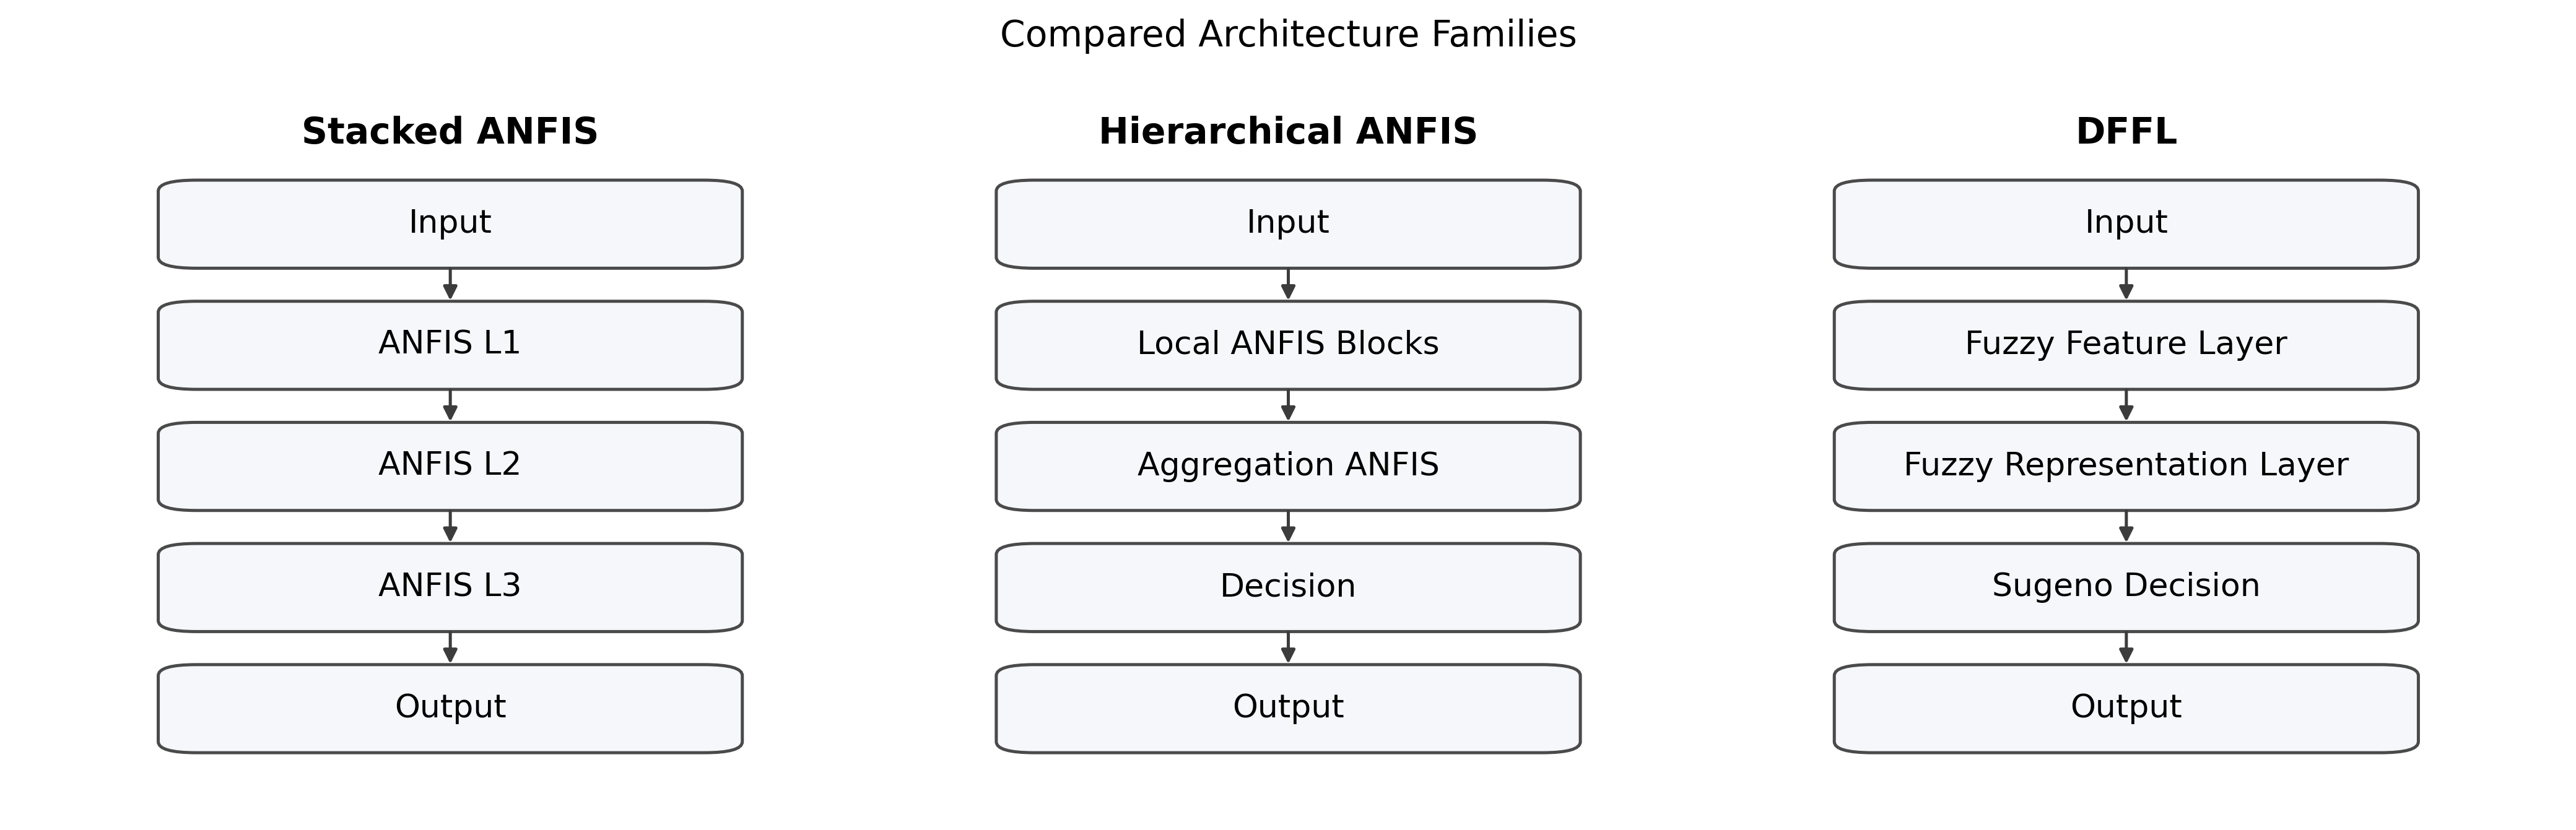
\includegraphics[width=\textwidth]{fig1_architectures.png}}
    \caption{Overview of the four model families considered in the study: shallow, stacked, hierarchical, and DFFL.}
    \label{fig:architectures_overview}
\end{figure}

For a rule $r$ in a fuzzy block, the activation weight is defined as
\[
w_r = \sigma(g_r)\prod_{(i,j)\in A_r}\mu_{ij}(z_i),
\]
where $A_r$ denotes the antecedent structure of the rule, $\mu_{ij}(z_i)$ is the membership degree of the corresponding variable, and $\sigma(g_r)$ is a learnable rule gate. The gate is sample-independent and controls the global availability of rule $r$, while the product term is sample-dependent and encodes instance-specific antecedent matching. The activations are normalized as
\[
\bar{w}_r = \frac{w_r}{\sum_q w_q + \varepsilon},
\]
which keeps rule contributions comparable and numerically stable during training.

The same normalized activations are used to form either hidden concept representations or the final output. In hidden layers, the concept representation may be written as
\[
c = \sum_r \bar{w}_r v_r,
\]
where $z\in \mathbb{R}^{m}$ is the block input, $c\in\mathbb{R}^{k}$ is the block output, and $v_r\in\mathbb{R}^{k}$ is the concept vector associated with rule $r$. In a more expressive variant, the hidden consequent is parameterized as
\[
c = \sum_r \bar{w}_r \sigma(zW_r + b_r).
\]
Here $W_r\in\mathbb{R}^{m\times k}$ and $b_r\in\mathbb{R}^{k}$.
At the final stage, prediction is produced by a first-order Sugeno mapping,
\[
\hat{y} = \sum_r \bar{w}_r \left(a_{r0} + a_r^\top z\right),
\]
where $z$ denotes the representation at the last hidden level.

The shallow model serves as the reference configuration. It uses a single fuzzy block over the full input space and a single decision layer. Its main advantage is local readability, since the rule base remains relatively easy to inspect. Its limitation is restricted representational depth.

In the stacked model, depth is introduced through a sequential composition of fuzzy blocks. The output of one block becomes the input to the next. This design refines the representation step by step and often improves predictive performance, but the resulting intermediate states may become technical latent transformations rather than semantically stable concepts.

In the hierarchical model, depth is introduced through decomposition rather than simple sequential stacking. Local groups of features are processed by separate fuzzy blocks, and their outputs are then aggregated at a higher level. This reduces the pressure on a single global rule base and provides a more controlled compromise between predictive performance and structural complexity. However, hierarchical organization alone does not guarantee semantically transparent intermediate states.

DFFL differs from both designs by treating hidden levels as concept-oriented fuzzy representations rather than generic latent transformations. Local fuzzy blocks first construct concept-level states, which are then aggregated and refined before the final decision stage. In this architecture, depth increases expressive power and preserves a traceable internal reasoning path from input features to the final prediction. A schematic representation of DFFL is shown in Fig.~\ref{fig:dffl_architecture}.

The technical distinction between DFFL and hierarchical ANFIS is the explicit two-stage concept flow with a separate global aggregation and refinement stage before the decision layer. Hierarchical ANFIS decomposes input processing, but does not enforce this concept-flow constraint or the same staged re-estimation path. In this study, DFFL also uses concept-stage re-estimation before final joint training, which is not reproduced in the stacked and hierarchical configurations.

For clarity, we write the four architectures as explicit mappings built from fuzzy blocks $F(\cdot)$ with the shared inference equations above. Shallow uses one block and a decision map,
\[
\hat{y}_{\mathrm{shallow}} = D\!\left(F_1(x)\right).
\]
Stacked uses sequential composition,
\[
z^{(0)}=x,\quad z^{(\ell)} = F_{\ell}\!\left(z^{(\ell-1)}\right),\ \ell=1,\dots,L,\quad
\hat{y}_{\mathrm{stacked}} = D\!\left(z^{(L)}\right).
\]
Hierarchical uses grouped local processing and top aggregation,
\[
h_g = F_g\!\left(x_{\mathcal{G}_g}\right),\ g=1,\dots,G,\quad
\hat{y}_{\mathrm{hier}} = D\!\left(A\!\left(h_1,\dots,h_G\right)\right).
\]
DFFL uses local concept extraction, aggregate concept construction, and global refinement before decision,
\[
c_g^{(1)} = F_g^{\mathrm{loc}}\!\left(x_{\mathcal{G}_g}\right),\quad
c^{(2)} = A_{\mathrm{concept}}\!\left(c_1^{(1)},\dots,c_G^{(1)}\right),\quad
\hat{y}_{\mathrm{DFFL}} = D\!\left(R\!\left(c^{(2)}\right)\right).
\]

\begin{figure}[H]
    \centering
    \IfFileExists{2.jpg}
        {\includegraphics[width=\textwidth]{2.jpg}}
        {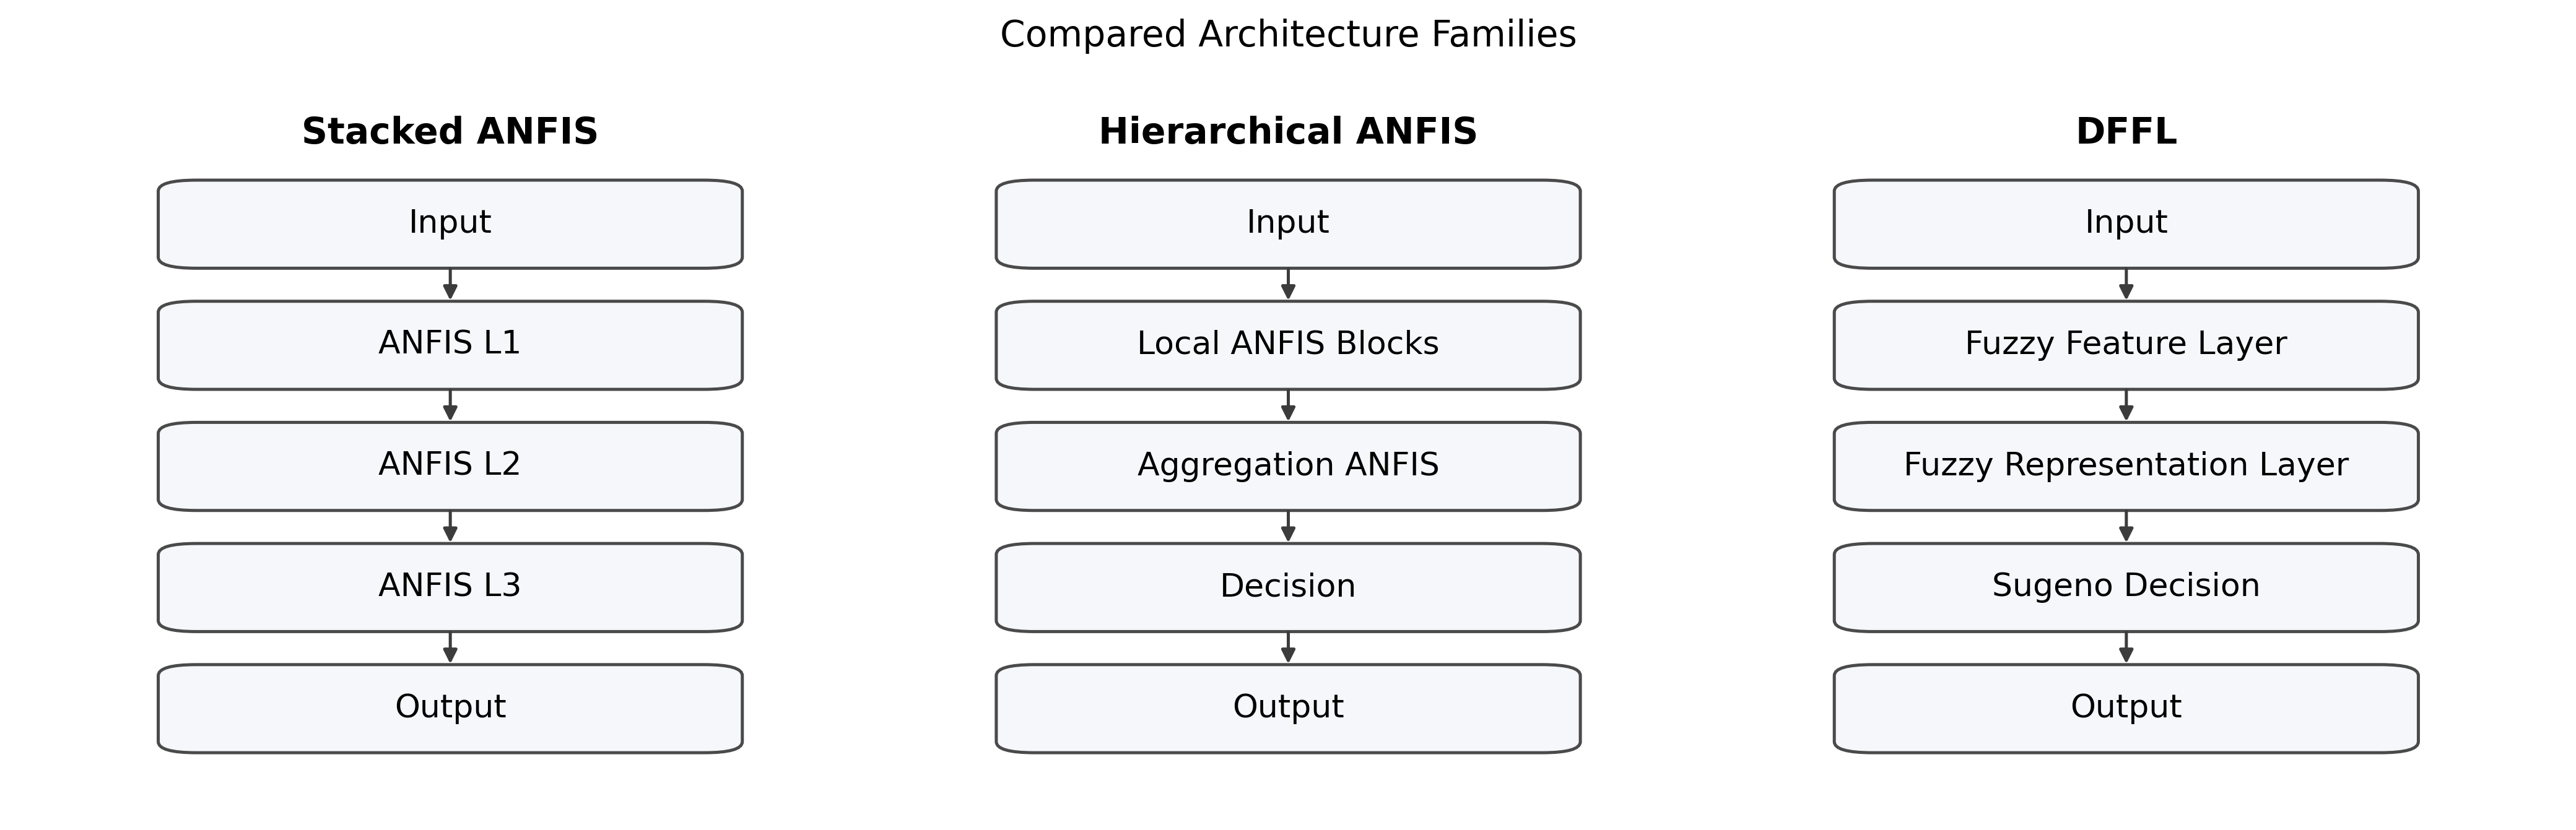
\includegraphics[width=\textwidth]{fig1_architectures.png}}
    \caption{Detailed architecture of DFFL with local concept blocks, aggregate concept layers, global refinement, and the final decision layer.}
    \label{fig:dffl_architecture}
\end{figure}

Structural complexity is treated as an explicit architectural property rather than as a secondary implementation detail. In a flat global rule base, the number of candidate rules grows rapidly with input dimensionality. Local processing and restricted rule length reduce this growth and make it possible to analyze complexity as a measurable structural cost.

Training is performed within a unified optimization framework, but DFFL is considered in two regimes. In the one-phase regime, all trainable components are optimized jointly after initialization. In the refined regime, training is staged: initialization is followed by concept-level pretraining, rule-base re-estimation in the updated representation space, and final fine-tuning. The purpose of this staged procedure is to stabilize the internal representation and make the hidden rule structure more reproducible across runs.

The overall objective combines task performance with structural regularization,
\[
\mathcal{L} =
\mathcal{L}_{\mathrm{task}}
+ \lambda_{\mathrm{s}}\mathcal{L}_{\mathrm{sparse}}
+ \lambda_{\mathrm{l}}\mathcal{L}_{\mathrm{len}}
+ \lambda_{\mathrm{ord}}\mathcal{L}_{\mathrm{order}}
+ \lambda_{\mathrm{ov}}\mathcal{L}_{\mathrm{overlap}}
+ \lambda_{\mathrm{c}}\mathcal{L}_{\mathrm{cover}}
+ \lambda_{\mathrm{ort}}\mathcal{L}_{\mathrm{orth}}
+ \lambda_{\mathrm{b}}\mathcal{L}_{\mathrm{bin}}
+ \lambda_{\mathrm{g}}\mathcal{L}_{\mathrm{gate}}.
\]
Here, $\mathcal{L}_{\mathrm{task}}$ corresponds to the predictive objective, while the remaining terms impose structural constraints related to sparsity, rule length, ordering, overlap control, coverage, concept separation, binarization, and gate usage. Under this formulation, interpretability is encouraged directly during learning rather than added as a post hoc explanation.

The refined DFFL training procedure used in this study starts with initialization of local, aggregate, and decision blocks from data-driven prototypes and predefined rule budgets. After that, we run stage-wise pretraining of concept blocks on the training split, then re-estimate rule candidates in the updated concept spaces and rebuild active block structures. Next, we pretrain the decision layer on fixed concept features and then run joint fine-tuning of all trainable parameters with the unified objective and early stopping. For binary tasks, the final classification threshold is tuned on the validation split.
This staged procedure is specific to DFFL in this paper. Shallow, stacked, and hierarchical models are trained without concept-stage re-estimation.

The empirical evaluation was designed to compare the considered architectures within a unified experimental framework. The benchmark includes tabular regression and binary classification tasks, with a main comparison block on smaller standard data sets and an extended comparison block on larger data sets. For large-scale analysis, we use full \textit{covtype\_binary} as the main discriminative benchmark and \textit{kddcup99\_binary\_10percent} as a feasibility/scalability check with repeated-run stability reporting. We also report an additional discriminative large-scale check on \textit{SUSY-200k}.

Reproducibility settings are fixed as follows: three seeds ($19,23,29$), test split $0.2$, validation split $0.2$ (from the original data), feature scaling by MinMax normalization to $[0,1]$, and target scaling to $[0,1]$ for regression tasks. The same seed-specific data split is used for all compared models.

For regression tasks, predictive quality is assessed by the root mean squared error (RMSE). For binary classification, the main metric is the F1 score. Since the study addresses predictive accuracy together with interpretable depth, the evaluation also includes structural and stability-oriented measures. In particular, we record the total number of rules, the number of active rules, and the Jaccard similarity of active-rule configurations across repeated runs.

The comparison includes the four neuro-fuzzy architectures introduced above. To place their predictive performance in a broader context, we also include standard machine-learning baselines, including linear models, random forests, multilayer perceptrons, Extra Trees, and Histogram Gradient Boosting.

For fuzzy models, the optimization budget is controlled by common defaults: pretraining epochs $18$, decision-pretraining epochs $14$, maximum epochs $80$, patience $20$, and batch size $64$. In binary tasks, the default classification threshold is $0.5$ and can be tuned on validation data in $[0.05,0.95]$. Hyperparameters are selected on validation splits under fixed family-specific search spaces and fixed trial budgets. For fairness, all compared models within each run use the same seed-specific split and fixed per-family budget policies. Standard ML baselines are evaluated on the same splits with fixed model configurations. Resolved settings, including regularization coefficients, are reported in the reproducibility artifacts.

A structured reproducibility package is provided with the manuscript materials and includes resolved run configurations, seeds, metric tables, and figure-generation inputs (\href{https://github.com/lebedeffson/deep-neuro-fuzzy/tree/main/docs/article_current}{article bundle}, \href{https://github.com/lebedeffson/deep-neuro-fuzzy/tree/main/docs/artifacts}{artifacts}).

In this paper, interpretability is operationalized as \textit{structural interpretability}. It is evaluated at two complementary levels. The first is global and concerns the stability of the internal rule structure across repeated runs. The second is local and concerns the decision path for an individual test object. Together, these two perspectives assess reproducibility and traceability of the internal reasoning process. We do not treat this protocol as a full semantic interpretability validation.

At the global level, interpretability is analyzed through the Jaccard similarity of active rules and decision-layer rules across independent runs. For run $s$, a rule is considered active if $p_r^{(s)}\ge \tau_{\mathrm{act}}$, where $p_r^{(s)}$ is the learned rule probability and $\tau_{\mathrm{act}}=0.5$. If $R_a$ and $R_b$ are active-rule sets from two runs, then
\[
J(R_a,R_b)=\frac{|R_a\cap R_b|}{|R_a\cup R_b|}.
\]
These quantities show whether an architecture tends to recover a stable internal structure rather than a substantially different rule configuration at each training instance. We use this metric as a structural stability proxy and not as a full semantic interpretability measure.

At the local level, interpretability is examined through a case-level analysis of a single test object. The procedure follows a fixed sequence: input object, membership values, most active first-level rules, aggregated concept states, decision-layer rules, and final output. Figure~\ref{fig:case_explainability_flow} illustrates this logic.

To improve semantic readability beyond index-level tracing, hidden concept indices are mapped to their originating feature groups and original feature names in the case-level supplementary artifact.

\begin{figure}[H]
    \centering
    \IfFileExists{3.jpg}
        {\includegraphics[width=\textwidth]{3.jpg}}
        {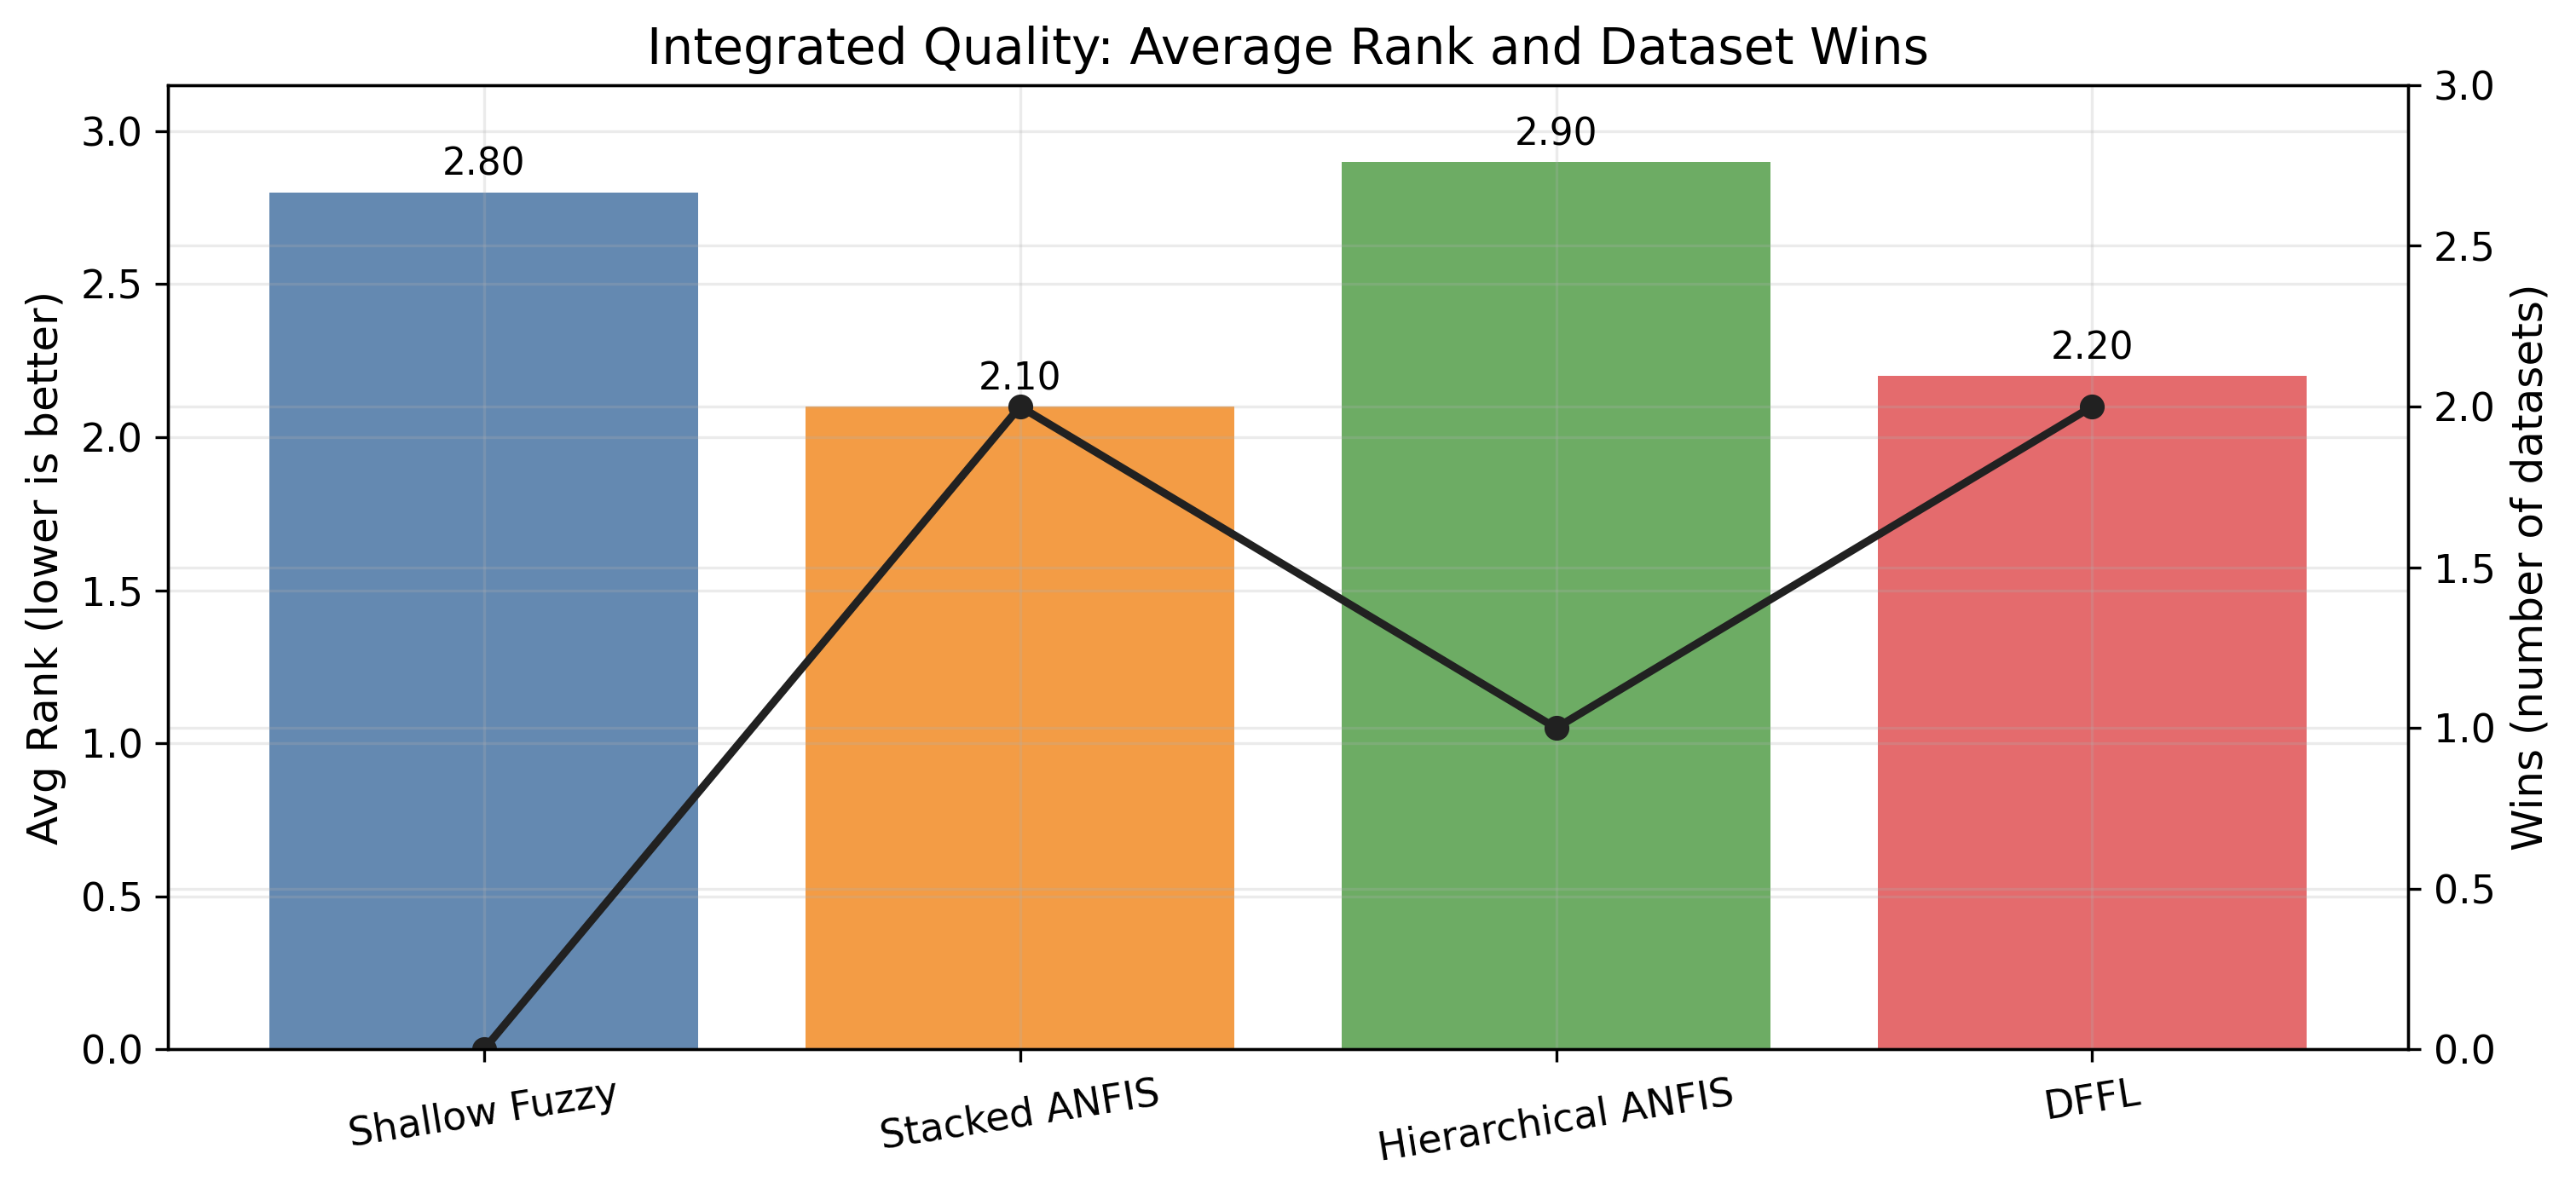
\includegraphics[width=\textwidth]{fig3_rank_and_wins.png}}
    \caption{Case-level explainability flow in DFFL: from the input object through membership values and the most active first-level rules to aggregated concepts, decision rules, and the final output.}
    \label{fig:case_explainability_flow}
\end{figure}

In the present study, the local analysis is demonstrated on a correctly classified example from the \textit{breast\_cancer} data set. For this object, DFFL produces a probability of 0.0028 for the positive class and a logit of $-5.8650$, which corresponds to the correct prediction of class~0. The first level of the architecture is dominated by a small number of strong local rules, showing that the input is processed through a compact set of salient antecedent patterns rather than through a diffuse set of weak activations. At the next level, these local signals are compressed into aggregate concept states, so that the decision path becomes progressively more structured and less redundant. By the time the model reaches the output layer, the final prediction is determined by a small group of dominant decision rules that together produce a strongly negative logit.

The dominant rules involved in this example are summarized in Table~\ref{tab:case_rules}.

\begin{table}[H]
\centering
\caption{Dominant rules in the case-level example for DFFL.}
\label{tab:case_rules}
\small
\setlength{\tabcolsep}{4pt}
\begin{tabular}{lcll}
\toprule
Level & Rule & Weight & Role \\
\midrule
Stage 1 & \texttt{x1 IS mid AND x3 IS mid} & 0.7774 & dominant local signal \\
Stage 1 & \texttt{x6 IS mid AND x7 IS mid} & 0.9987 & nearly complete block activation \\
Stage 1 & \texttt{x20 IS mid AND x22 IS mid} & 0.9940 & stable local concept \\
Stage 2 & \texttt{s1\_15 IS high AND s1\_17 IS low} & 0.7889 & main aggregate transition \\
Stage 2 & \texttt{s1\_18 IS low AND s1\_19 IS high} & 0.8739 & dominant global state \\
Decision & \texttt{s2\_0 IS low AND s2\_5 IS low} & 0.3554 & strongest negative contribution \\
Decision & \texttt{s2\_0 IS low AND s2\_1 IS low} & 0.3111 & second strongest contribution \\
Decision & \texttt{s2\_4 IS high AND s2\_5 IS low} & 0.0959 & complementary decision signal \\
\bottomrule
\end{tabular}
\end{table}

Taken together, the global stability analysis and the local case-level trace define a unified interpretability protocol for the compared models. The former shows whether an architecture tends to recover a reproducible internal rule structure across runs, while the latter shows whether this structure can be read as a coherent decision path for an individual object.

\section{Results}

The compared architectures differ along three evaluation dimensions: predictive quality, rule-base complexity, and internal rule stability. In the main comparison block, stacked shows the strongest average-rank profile, while DFFL remains competitive on selected tasks and no architecture dominates all tasks at once.
The key quantitative evidence is reported in Tables~\ref{tab:main_results}, \ref{tab:extended_results}, \ref{tab:covtype_capacity_check}, \ref{tab:susy_discriminative}, \ref{tab:best_vs_baseline}, and \ref{tab:all_vs_baseline}. The quality profile across tasks is shown in Fig.~\ref{fig:quality_main}, and the quality--complexity--stability trade-off for the main block is shown in Fig.~\ref{fig:complexity_stability}.
Values in Tables~\ref{tab:main_results}--\ref{tab:all_vs_baseline} are reported as mean $\pm$ standard deviation across three seeds, except entries explicitly marked as single-seed checks; complete run settings and outputs are provided in the reproducibility artifacts.
For transparency, Table~\ref{tab:main_results} uses one unified reference run for all four neuro-fuzzy architectures under matched seeds, splits, preprocessing, and training budget.

\begin{table}[H]
\centering
\caption{Summary results of the compared architectures in the main comparison block (mean $\pm$ std over three seeds).}
\label{tab:main_results}
\scriptsize
\setlength{\tabcolsep}{1.5pt}
\begin{tabular}{lllccccc}
\toprule
Model & Avg. rules & \makecell[c]{Mean active-rule\\Jaccard} & Diabetes & Linnerud weight & Breast cancer & Wine binary & Digits binary\\
 &  &  & RMSE & RMSE & F1 & F1 & F1 \\
\midrule
shallow model      & 36.00 & 0.2352 & 0.1852$\pm$0.0024 & 0.3519$\pm$0.2209 & 0.9750$\pm$0.0085 & 0.9577$\pm$0.0340 & 0.9367$\pm$0.0141 \\
stacked model      & 50.00 & 0.1268 & 0.1857$\pm$0.0035 & 0.2887$\pm$0.1396 & 0.9841$\pm$0.0064 & 0.9855$\pm$0.0205 & 0.9953$\pm$0.0066 \\
hierarchical model & 75.00 & 0.1766 & 0.1937$\pm$0.0051 & 0.2430$\pm$0.1691 & 0.9722$\pm$0.0102 & 0.9189$\pm$0.0327 & 0.9953$\pm$0.0066 \\
DFFL               & 75.47 & 0.0888 & 0.1796$\pm$0.0032 & 0.2874$\pm$0.2340 & 0.9652$\pm$0.0207 & 0.9564$\pm$0.0372 & 1.0000$\pm$0.0000 \\
\bottomrule
\end{tabular}
\end{table}

\begin{figure}[H]
    \centering
    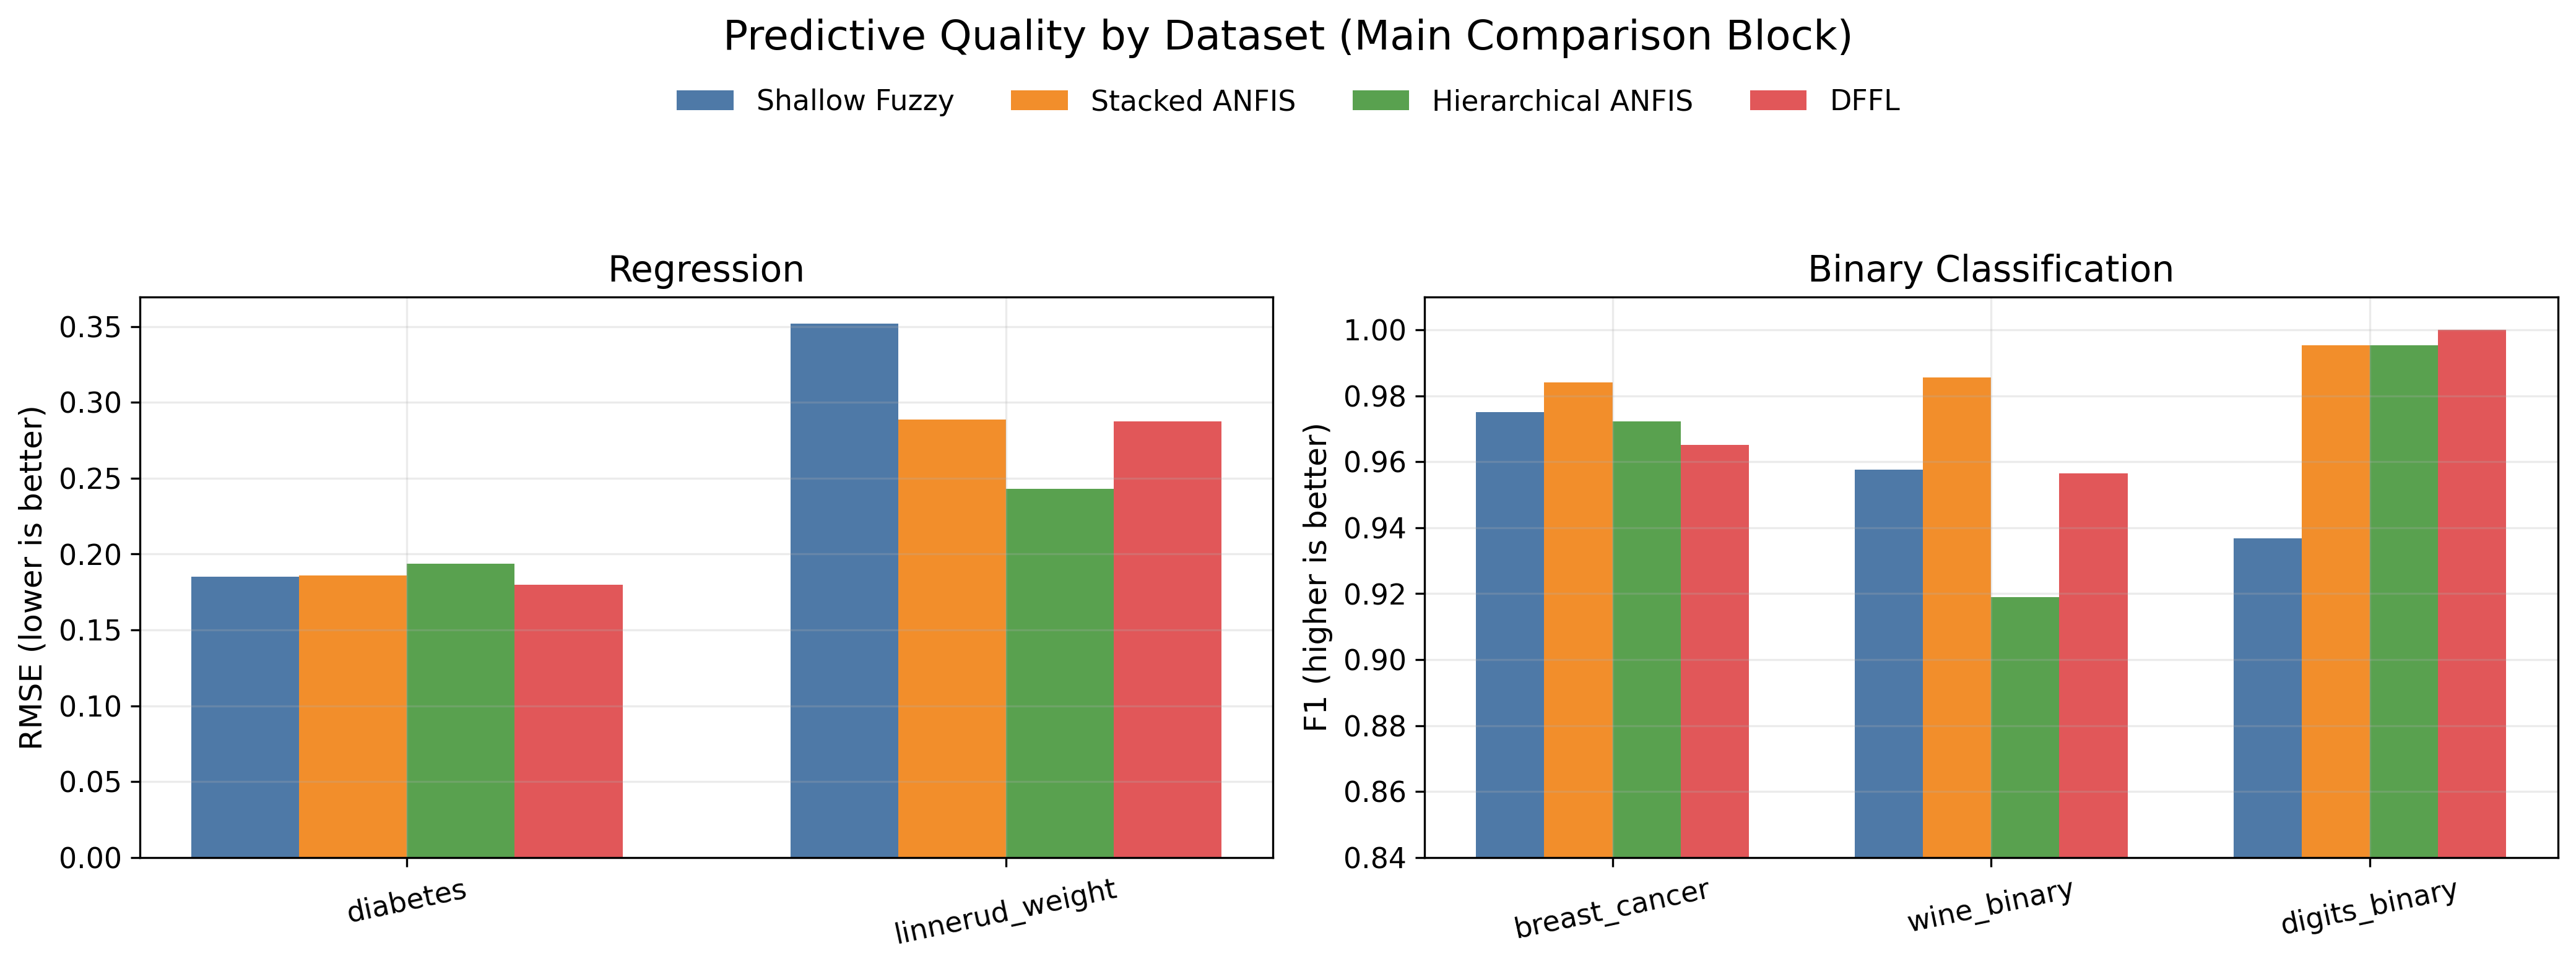
\includegraphics[width=\textwidth]{fig2_quality_by_dataset.png}
    \caption{Predictive quality of the compared models in the main comparison block.}
    \label{fig:quality_main}
\end{figure}

The extended comparison shows the same pattern: stacked and hierarchical remain the strongest predictive variants, while DFFL remains below these two models on the larger Covtype benchmark in the fixed three-seed verification setting.

\begin{table}[H]
\centering
\caption{Summary results of the compared architectures in the extended comparison (mean $\pm$ std over three seeds).}
\label{tab:extended_results}
\small
\setlength{\tabcolsep}{6pt}
\begin{tabular}{lcccc}
\toprule
Model & Avg. rules & \makecell[c]{Mean active-rule\\Jaccard} & California housing & Covtype binary \\
 &  &  & RMSE & F1 \\
\midrule
shallow model      & 36  & 0.3841 & 0.1321$\pm$0.0010 & 0.7101$\pm$0.0183 \\
stacked model      & 50  & 0.1559 & 0.1193$\pm$0.0066 & 0.8129$\pm$0.0108 \\
hierarchical model & 90  & 0.2343 & 0.1233$\pm$0.0044 & 0.8117$\pm$0.0052 \\
DFFL               & 115.67 & 0.2712 & 0.1285$\pm$0.0013 & 0.7518$\pm$0.0046 \\
\bottomrule
\end{tabular}
\end{table}

After the hard-finetune safety fix (validation-based keep/rollback), we additionally re-ran a focused three-seed check on \textit{covtype\_binary\_20000}. The ranking remained unchanged: stacked F1 $=0.8222\pm0.0074$, hierarchical F1 $=0.8037\pm0.0058$, DFFL F1 $=0.7840\pm0.0078$, and shallow F1 $=0.7645\pm0.0030$. Thus, the implementation fix improves reliability of training behavior without changing the main comparative conclusion on this data regime.

When the analysis shifts from predictive quality to internal rule stability, the picture changes. In the current quality-oriented DFFL setting, active-rule Jaccard in the main block is lower than in the strongest stability-oriented variants, which indicates that quality-focused tuning can reduce reproducibility of internal active-rule configurations.

Because the larger Covtype task suggested that the reference stacked model may be capacity-limited, we additionally ran a targeted large-scale capacity check on the full \textit{covtype\_binary} data set with 581,012 samples. This check is reported separately from the unified reference comparison because it uses an enhanced stacked configuration: larger hidden width and rule budget (factor $3.0$), a gated final skip from 32 selected raw features, distillation from an Extra Trees teacher (blend weight $0.15$), and a second-stage error-focused fine-tuning. The result is a stronger stacked variant with 150 rules and 33 hidden concepts.

\begin{table}[H]
\centering
\caption{Large-scale results on full \textit{covtype\_binary} (three-seed results).}
\label{tab:covtype_capacity_check}
\scriptsize
\setlength{\tabcolsep}{4pt}
\begin{tabular}{lccccc}
\toprule
Model & F1 & ROC-AUC & PR-AUC & Rules & Active-rule Jaccard \\
\midrule
stacked (enhanced configuration) & 0.9466$\pm$0.0015 & 0.9895$\pm$0.0005 & 0.9886$\pm$0.0005 & 150 & 0.1625 \\
DFFL & 0.8478$\pm$0.0037 & 0.9246$\pm$0.0033 & 0.9149$\pm$0.0037 & 144 & 0.0222 \\
hierarchical (enhanced configuration) & 0.8930$\pm$0.0004 & 0.9615$\pm$0.0009 & 0.9573$\pm$0.0013 & 207 & 0.2050 \\
hist gradient boosting & 0.8328$\pm$0.0011 & 0.9183$\pm$0.0010 & 0.9099$\pm$0.0012 & -- & -- \\
MLP & 0.8589$\pm$0.0009 & 0.9377$\pm$0.0026 & 0.9307$\pm$0.0029 & -- & -- \\
extra trees & 0.9543$\pm$0.0003 & 0.9919$\pm$0.0001 & 0.9912$\pm$0.0002 & -- & -- \\
random forest & 0.9560$\pm$0.0001 & 0.9924$\pm$0.0001 & 0.9918$\pm$0.0001 & -- & -- \\
\bottomrule
\end{tabular}
\end{table}

The capacity-tuned stacked model substantially improves over the smaller reference configurations and becomes stronger than histogram gradient boosting, MLP, and the tested hierarchical fuzzy variant on full Covtype. However, it remains below Random Forest and Extra Trees. DFFL in the current three-seed run reaches F1 $=0.8478\pm0.0037$, which is above histogram gradient boosting but below MLP, stacked, and tree ensembles.

As an additional fairness-oriented diagnostic, we ran a capacity-matched fuzzy-only setting on full Covtype under a unified fast budget. In this setting, stacked and DFFL use near-matched total rules (106 and 107 respectively), while hierarchical uses 171 rules in the same budget regime. Stacked remains the strongest fuzzy variant (F1 $=0.9049\pm0.0043$), followed by hierarchical (F1 $=0.8540\pm0.0051$) and DFFL (F1 $=0.8021\pm0.0075$). This diagnostic indicates that, in the current implementation, DFFL does not close the quality gap to stacked even when the rule-budget comparison is constrained.

As a secondary large-scale sanity check, we evaluate \textit{kddcup99\_binary\_10percent}. This setting confirms feasibility and repeated-run stability, but it is weakly discriminative because most methods approach perfect scores. For this reason, we do not use KDD as a primary quality separator in the main comparative interpretation.

To reduce the near-perfect saturation effect observed on KDD, we add a more discriminative large-scale check on \textit{SUSY-200k}. Fuzzy-model values are reported over three seeds, while baseline values are a single-seed snapshot (seed 23) and are therefore treated as contextual rather than significance-tested comparisons.

\begin{table}[H]
\centering
\caption{Additional discriminative large-scale check on \textit{SUSY-200k}.}
\label{tab:susy_discriminative}
\scriptsize
\setlength{\tabcolsep}{4pt}
\begin{tabular}{lcccc}
\toprule
Model & F1 & ROC-AUC & PR-AUC & Seeds \\
\midrule
shallow fuzzy & 0.7626$\pm$0.0062 & 0.8582$\pm$0.0072 & 0.8602$\pm$0.0092 & 3 \\
stacked fuzzy & 0.7713$\pm$0.0039 & 0.8685$\pm$0.0039 & 0.8725$\pm$0.0042 & 3 \\
hierarchical fuzzy & 0.7708$\pm$0.0047 & 0.8688$\pm$0.0032 & 0.8738$\pm$0.0028 & 3 \\
DFFL & 0.7718$\pm$0.0020 & 0.8688$\pm$0.0021 & 0.8728$\pm$0.0015 & 3 \\
logistic regression & 0.7395 & 0.8556 & 0.8595 & 1 \\
hist gradient boosting & 0.7655 & 0.8745 & 0.8789 & 1 \\
mlp classifier & 0.7687 & 0.8736 & 0.8787 & 1 \\
\bottomrule
\end{tabular}
\end{table}

To evaluate robustness, we report nonparametric tests on benchmark summaries: a Friedman test with pairwise Wilcoxon signed-rank tests and Holm correction. In the main block, the dataset-level Friedman test is not significant ($\chi^2=2.04$, $p=0.6327$). In the extended block, it is significant ($\chi^2=6.00$, $p=0.0383$), but no pairwise comparison remains significant after Holm correction at $\alpha=0.05$.
These tests are computed on the unified three-seed benchmark blocks, while the separate full-Covtype capacity table is treated as a diagnostic and excluded from significance testing.

Because active-rule stability depends on the activation threshold $\tau_{\mathrm{act}}$, we additionally ran a threshold-sensitivity check on the main benchmark block with $\tau\in\{0.3,0.5,0.7\}$. At $\tau=0.3$, mean active-rule Jaccard across datasets is 0.4511 (stacked), 0.4381 (hierarchical), and 0.2261 (DFFL). At the default $\tau=0.5$, the same values are 0.1218, 0.1640, and 0.2198. At $\tau=0.7$, stacked and hierarchical saturate at 1.0 in this fast setting due to the very sparse surviving active-rule sets, while DFFL remains at 0.2090. This supplementary fast-setting check is threshold-sensitive and does not replace the main reference comparison in Table~\ref{tab:main_results}. We therefore keep $\tau_{\mathrm{act}}=0.5$ as the default reporting point and interpret high-$\tau$ values with caution.

The comparison with external baselines is included only to contextualize raw predictive performance. The main contribution of this study is the comparative analysis of neuro-fuzzy architectures in terms of predictive quality, rule-base complexity, and internal rule stability.

\begin{table}[H]
\centering
\caption{Neuro-fuzzy results in the context of standard ML baselines (mean $\pm$ std over three seeds)}
\label{tab:best_vs_baseline}
\scriptsize
\setlength{\tabcolsep}{3pt}
\begin{tabular}{lclclc}
\toprule
Dataset & Metric & Best neuro-fuzzy model & Value & Best baseline & Value \\
\midrule
diabetes               & RMSE & DFFL               & 0.1796$\pm$0.0032 & linear regression                 & 0.1779$\pm$0.0025 \\
linnerud\_weight       & RMSE & hierarchical model & 0.2430$\pm$0.1691 & hist gradient boosting regressor & 0.3058$\pm$0.1508 \\
breast\_cancer         & F1   & stacked model      & 0.9841$\pm$0.0064 & extra trees classifier           & 0.9908$\pm$0.0032 \\
wine\_binary           & F1   & stacked model      & 0.9855$\pm$0.0205 & extra trees classifier           & 1.0000$\pm$0.0000 \\
digits\_binary         & F1   & DFFL               & 1.0000$\pm$0.0000 & mlp classifier                   & 1.0000$\pm$0.0000 \\
california\_housing    & RMSE & stacked model      & 0.1193$\pm$0.0066 & hist gradient boosting regressor & 0.0972$\pm$0.0014 \\
covtype\_binary\_20000 & F1   & stacked model      & 0.8129$\pm$0.0108 & extra trees classifier           & 0.8546$\pm$0.0026 \\
\bottomrule
\end{tabular}
\end{table}

\begin{table}[H]
\centering
\caption{Each neuro-fuzzy architecture against the best external baseline per data set (signed delta; positive is better).}
\label{tab:all_vs_baseline}
\scriptsize
\setlength{\tabcolsep}{3pt}
\begin{tabular}{lclcccc}
\toprule
Dataset & Metric & Best baseline & Shallow & Stacked & Hierarchical & DFFL \\
\midrule
diabetes               & RMSE & linear regression                 & -0.0073 & -0.0079 & -0.0158 & -0.0017 \\
linnerud\_weight       & RMSE & hist gradient boosting regressor & -0.0462 & +0.0170 & +0.0628 & +0.0183 \\
breast\_cancer         & F1   & extra trees classifier           & -0.0159 & -0.0067 & -0.0186 & -0.0256 \\
wine\_binary           & F1   & extra trees classifier           & -0.0423 & -0.0145 & -0.0811 & -0.0436 \\
digits\_binary         & F1   & mlp classifier                   & -0.0633 & -0.0047 & -0.0047 & +0.0000 \\
california\_housing    & RMSE & hist gradient boosting regressor & -0.0349 & -0.0221 & -0.0262 & -0.0313 \\
covtype\_binary\_20000 & F1   & extra trees classifier           & -0.1444 & -0.0417 & -0.0428 & -0.1027 \\
\bottomrule
\end{tabular}
\end{table}

As shown in Table~\ref{tab:all_vs_baseline}, neuro-fuzzy models outperform the best external baseline on \textit{linnerud\_weight}. On the remaining tasks they are either below the baseline or at parity (\textit{digits\_binary} for DFFL).

\begin{figure}[H]
    \centering
    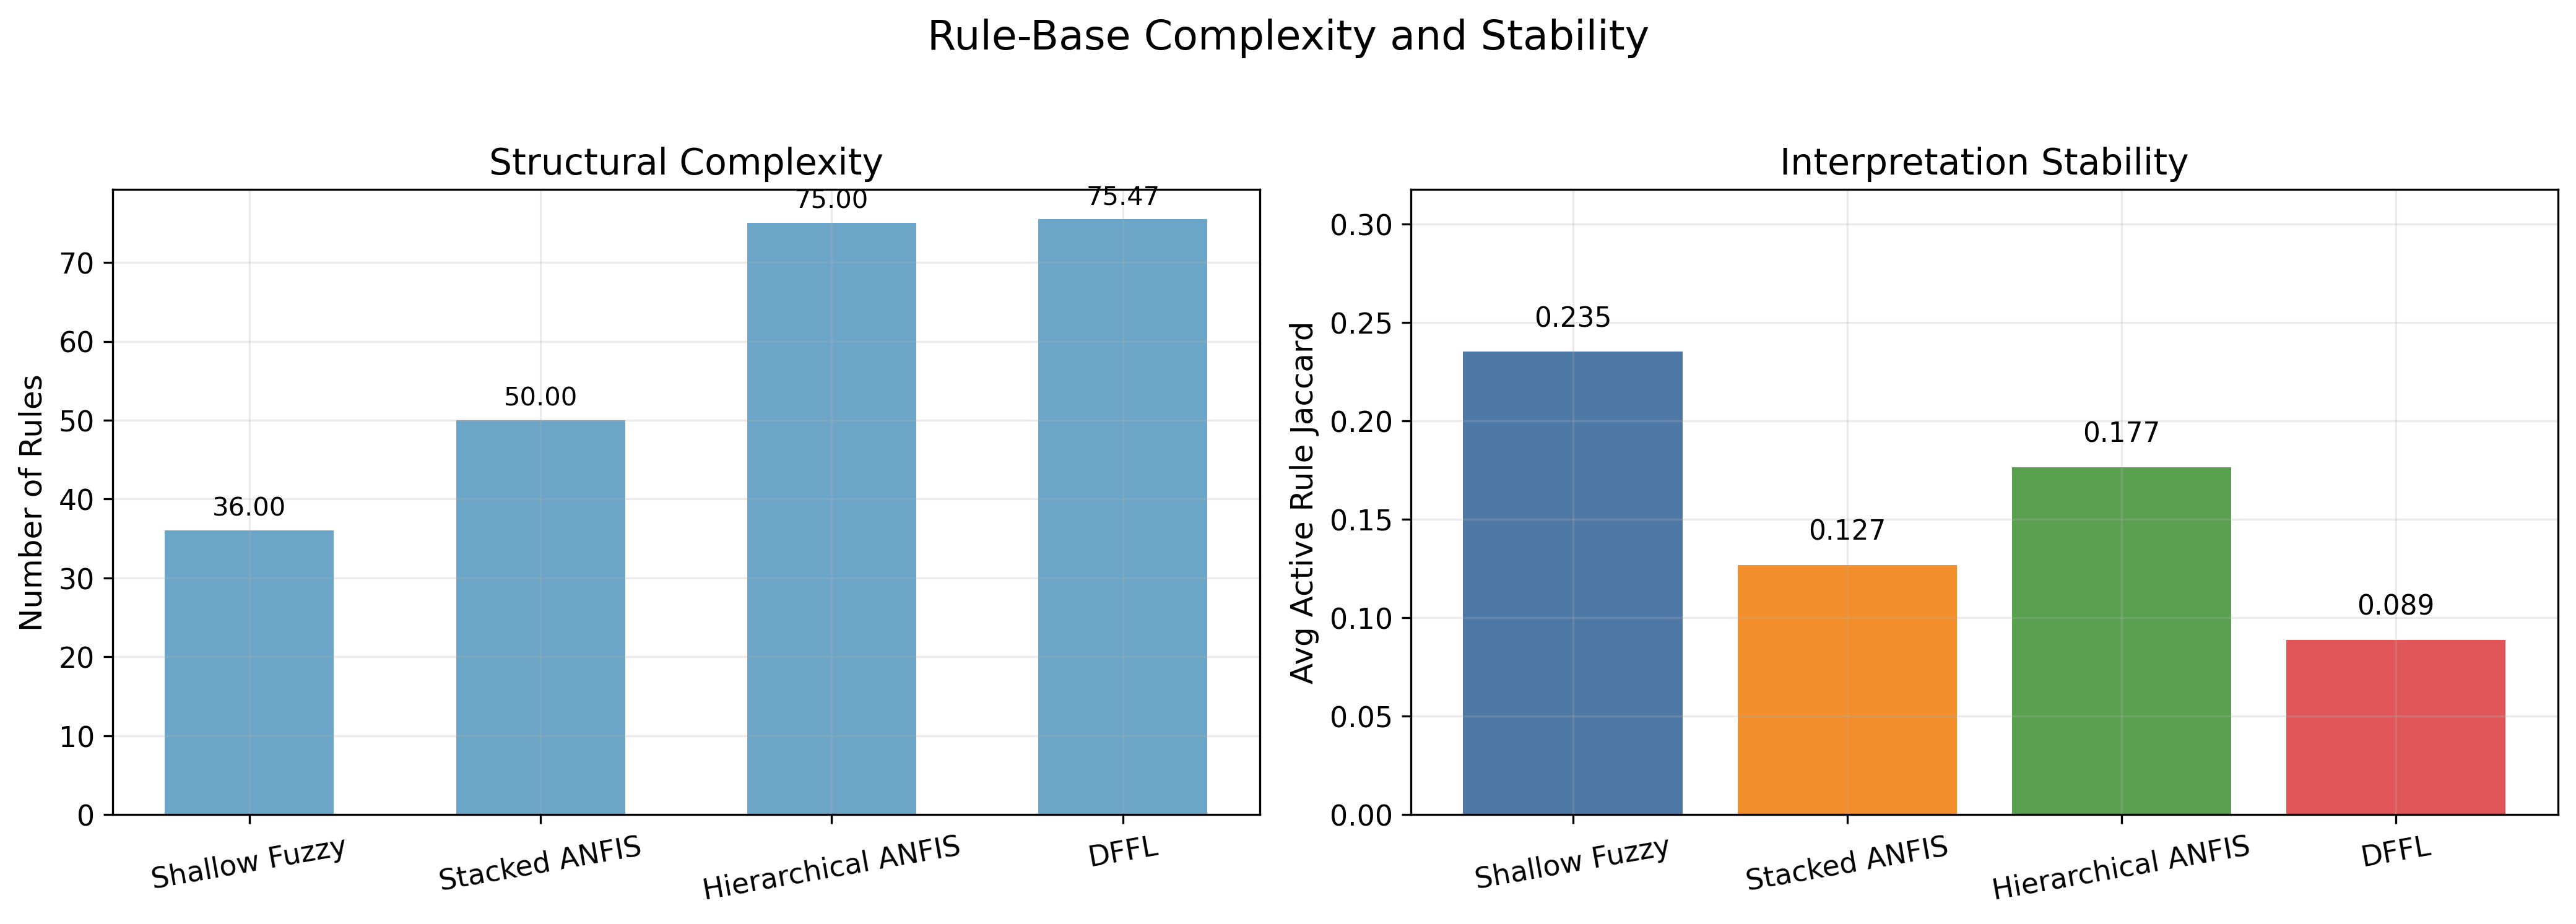
\includegraphics[width=\textwidth]{fig4_complexity_stability.png}
    \caption{Quality--complexity--stability trade-off across model families in the main comparison block.}
    \label{fig:complexity_stability}
\end{figure}

Overall, the results point to a trade-off rather than a single best architecture. Stacked leads the main block by average rank, while DFFL remains competitive and, in this quality-oriented profile, does not lead the active-rule stability metric.

The ablation of the DFFL training profiles leads to the same general conclusion. Quality-oriented profiles improve predictive quality on selected tasks and can control rule growth, but this may reduce active-rule reproducibility.

\section{Discussion}

The comparison shows a stable pattern. Different forms of depth in neuro-fuzzy systems support different objectives, and no single architecture dominates all criteria at once. Sequential and hierarchical organizations remain strong in predictive terms, especially in the extended block, while DFFL in the current quality-oriented setting stays competitive by rank but does not deliver the highest reproducibility of active internal rules.

The full Covtype capacity check clarifies this point at implementation level. The reference stacked setup was constrained by optimization settings and by the available rule and concept capacity. After increasing capacity and adding a gated raw-feature skip, stacked reached the strongest fuzzy result on this large task. At the same time, the gain required a larger rule budget and came with lower active-rule Jaccard, so the quality gain was achieved through a clear trade-off between quality, complexity, and stability.

Within the same Covtype setting, DFFL remains below the capacity-tuned stacked variant. This suggests that the current DFFL configuration still needs stronger bridge and aggregation capacity to preserve cross-feature information more effectively in high-dimensional tabular data.

Runtime measurements support the same interpretation. Under matched fast settings on full Covtype (seed 23), stacked was fastest in training at 69.57s, hierarchical was intermediate at 122.58s, and DFFL was slowest at 423.89s. Inference with evaluation remained in the same low-second range for all three methods, around 2--3s. In practical terms, DFFL currently pays both a quality penalty and a training-time penalty relative to stacked in the tested regime.

This is important for the main claim of the paper. If interpretability is treated as a property of internal reasoning rather than an external post hoc explanation, then evaluation cannot be reduced to RMSE or F1. Reproducibility of internal rule structure becomes a necessary criterion alongside predictive quality.

The current DFFL gains should therefore be read carefully. In these experiments, quality-oriented tuning improves ranking on selected tasks and gives the best fuzzy value on \textit{diabetes} (RMSE) and \textit{digits\_binary} (F1), but the model still stays below the strongest external baselines on most tasks and shows lower active-rule reproducibility. A reasonable interpretation is that concept-oriented depth can improve selected outcomes, yet it does not currently provide uniformly better efficiency.

One likely mechanism behind this trade-off is the early local decomposition used in DFFL. It reduces combinatorial rule growth, but it also creates an early information bottleneck because upper layers operate on aggregated local representations rather than the full original feature space. This design can weaken recovery of complex cross-feature interactions and helps explain the simultaneous pressure on predictive quality and rule-activation stability.

The baseline comparison reinforces the practical reading of the results. Standard machine-learning models often remain stronger in raw predictive metrics, while the value of the tested neuro-fuzzy architectures lies in how their structural design changes the balance between performance, structural cost, and interpretability-oriented stability.

\section{Limitations}

The main limitation is empirical scope. The current evidence is restricted to tabular tasks; extension to image, text, and other modalities requires dedicated validation under modality-specific pipelines.

The second limitation concerns semantic validation depth. In this paper, interpretability is evaluated primarily in structural terms through rule sets, rule counts, stability, and case-level traceability. This provides reproducible internal diagnostics, but full domain-expert assessment of concept meaning remains an important next stage.

The third limitation concerns current large-scale efficiency. In the reported setup, DFFL is not yet superior to the strongest stacked or tree-based alternatives on the largest tasks and requires more training time, which indicates clear optimization headroom for the current implementation.

\section{Conclusion}

This paper examined how to increase complexity in neuro-fuzzy models while preserving structural interpretability of internal reasoning. We developed, formalized, and implemented four ANFIS-based architectures in one framework and compared them under a unified protocol. The results show that different forms of depth lead to systematically different balances between predictive quality, structural complexity, and internal rule stability.

The study establishes DFFL as a concept-oriented ANFIS design with explicit staged concept flow and demonstrates, through controlled comparisons, where it is competitive and where capacity-tuned stacked configurations are stronger in raw predictive metrics. On full Covtype, the strongest fuzzy result is obtained by the enhanced stacked architecture, while DFFL exposes a different quality--complexity--stability regime.

These findings imply that architecture selection in deep neuro-fuzzy modeling should be treated as a joint optimization problem, where predictive accuracy, rule-base size, reproducibility of internal rule structure, and runtime efficiency are considered together.

Further work should improve structural and computational efficiency of concept-oriented deep fuzzy models, expand evaluation to broader data regimes, and strengthen semantic concept validation beyond structural stability metrics.

\bibliographystyle{splncs04}
\bibliography{references}

\end{document}
